\section{Kinect 2}

\subsection{Introduction}
The kinect 2 was developed by Microsoft for the Xbox One, however has since been made available to windows 8, or newer, users. This means that through the kinect 2 SDK, data from a kinect can be utilised for a much wider variety of functions. Within the current iteration of the tiberius project the kinect was used to collect depth data and perform standard deviation equations on this depth data so that a grid could be created that could be sent to the database and used by the A-Star algorithm. This depth data could be used to identify the best terrain to traverse, giving the best path for \gls{tiberius3}. Other data such as the original depth stream and a infra-red stream could also be sent to the web interface to be viewed while a mission was being done. The kinect can also provide a colour stream, figure \ref{fig:kinect-color}, that gives an image of what is in front of \gls{tiberius3}.

\begin{figure}[!htb]
\begin{center}
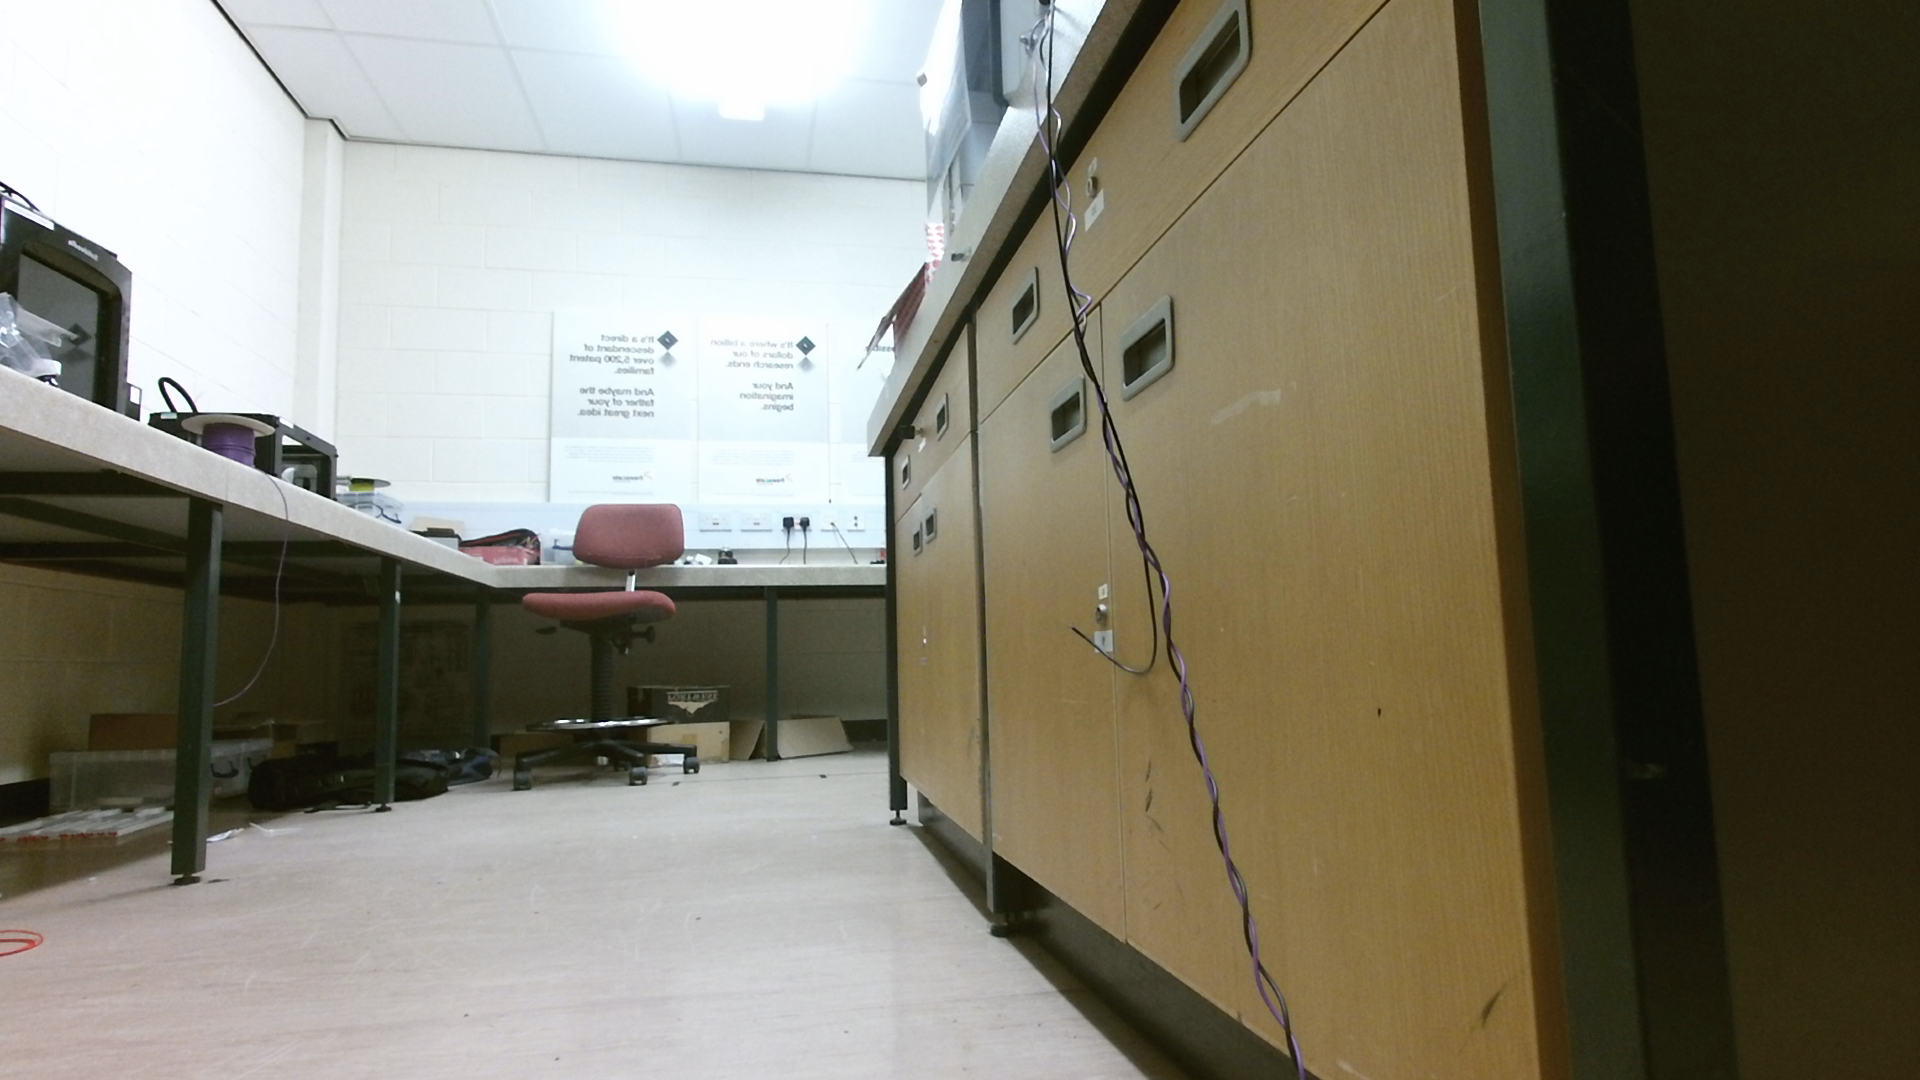
\includegraphics[width=10cm]{KinectScreenshot-Color.png}
\end{center}
\caption{Image produced by the kinect colour stream}
\label{fig:kinect-color}
\end{figure}

\subsection{Standard Deviation}\label{StandardDeviation}
The Kinect provides a range of useful data that can be used to created a wide range of data for different proposes. An example of this is to use the depth data to create a standard deviation grid that can be used for the A-Star algorithm within navigation for \gls{tiberius3}. This grid takes in the depth data that can be obtained from the Kinect and splits it into chunks as described in the next section \ref{Chunking} \textit{Chunking}. The data is then modified using the standard deviation equation that is seen in \ref{SDEquation}. The result can be seen in figure \ref{fig:sd-kinect}, a large pixel recreation of the depth data has been created. This can then be mapped to cells within the A-Star grid when performing the navigation algorithm in order to gain information about walls or terrain in front of \gls{tiberius3}.

\begin{figure}[!htb]
\begin{center}
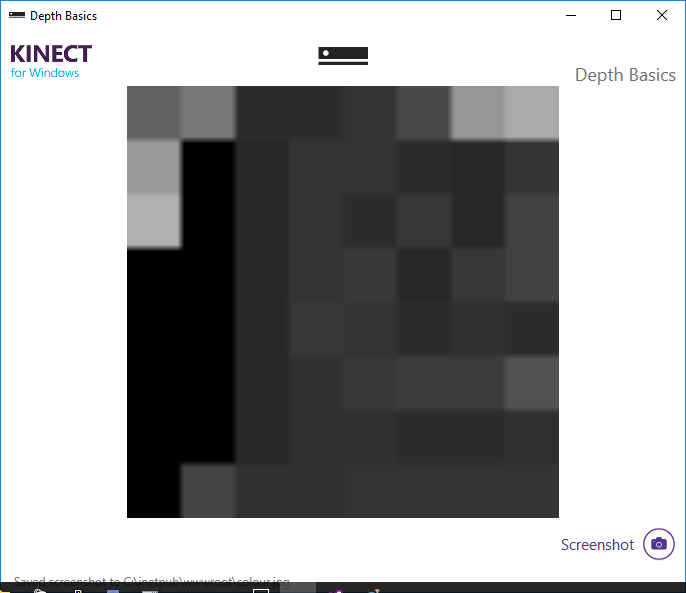
\includegraphics[width=10cm]{sd-kinect.png}
\end{center}
\caption{Image created by the kinect standard deviation stream created for this project}
\label{fig:sd-kinect}
\end{figure}

\begin{capequ}[!htb]
\begin{center}
\begin{equation}
\textit{SD} = \sqrt{\frac{\sum (x - x')^2}{N - 1}}
\end{equation}
\caption{Standard Deviation Equation}
\label{SDEquation}
\end{center}
\end{capequ}

\subsection{Chunking}\label{Chunking}
Chunking is the process of dividing a large dataset into several smaller ones. In our case this allowed us to split the depth image data that was received from the Kinect 2 and splitting it into an 8 by 8 grid. We could then perform the calculations on each element of the grid. The main reason for chunking our data was give us a much lower resolution image which was more useful and easily used on the control pi.

\subsection{Camera Streamer}
This C\# console application runs on the pc. It takes all the data coming from the Kinect 2 and processes it into a useful format.
The depth data is processed using the methods described in \ref{Chunking} \textit{Chunking} and \ref{StandardDeviation} \textit{Standard Deviation}. The colour, infra-red and depth streams are all downscaled to a lower resolution and then saved as JPEG image files on disk. Windows's built in web server IIS (Internet Information Services) then serves the image files to anyone that requests them.

\pagestyle{euanstuart}













